\documentclass[12pt]{article}

\usepackage{fullpage}
\usepackage{amsmath, amsthm, amssymb}
\usepackage{mathtools}
\usepackage{algorithm}
\usepackage[noend]{algpseudocode}
\usepackage{tikz}
\usetikzlibrary{topaths,calc}

\renewcommand{\algorithmicrequire}{\textbf{Input:}}
\renewcommand{\algorithmicensure}{\textbf{Output:}}

\makeatletter
\def\BState{\State\hskip-\ALG@thistlm}
\makeatother



\newtheorem{lemma}{Lemma}
\newtheorem{theorem}{Theorem}
\newtheorem{claim}{claim}
\newtheorem*{lemma*}{Lemma}
\newtheorem*{theorem*}{Theorem}
\newtheorem*{claim*}{Claim}

\title{On the Freshman Roommates Problem}
\author{Dominick Twitty (\texttt{dkt36})\\
\and Kelvin Luu (\texttt{kl583})\\
\and Jeff Tian (\texttt{yt336})
}
\date{}

\begin{document}
\maketitle

\begin{abstract}
In this document we discuss our experience generalizing matching problems to include arbitrary sets and numbers of agents per match. As a driving example, we use the problem of allocating freshmen students to dorm rooms of various sizes. In the binary version of this problem, we attempt to maximize the number of students compatibly housed, and in the rank-order version we attempt to generate Pareto-efficient allocations. We found that in general these problems are very difficult (NP-complete), so we propose heuristics that provide certain benefits while keeping reasonable runtime.  
\end{abstract}

\section*{Introduction}
Many matching problems involve one or two sets of agents, with each set having preferences for the other set. For example, in the College Admissions Problem, students have preferences for colleges and colleges have preferences for each individual student. Another example is the Stable Roommates Problem, in which there is one set of agents, each having preferences over the same set. We wanted to expand these problems with a mind for new and unusual situations. For instance, what if matchings can have any number of participants, or there are two sets of agents vying for the same properties?

We drive our exploration with the following problem: How do you optimally assign college freshmen to dorm rooms. This question is close to home - at Cornell, new students must live on campus, have minimal choice in \textit{which} room they get, and can put forth compatibility profiles in the hopes of finding a good roommate. Furthermore, rooms range in size from one to four people in the extreme case. Many freshmen end up loving (or at least tolerating) their roommate, but others would gladly switch with another. \textit{How can we provide students with better roommates?}

We propose two more formally defined problems, each related to the scenario above. First, given a list of students, the set of other students each one finds compatible, and a list of room sizes, we ask: \textbf{What room allocation maximizes the number of students compatibly housed?} This is the \textbf{Binary Freshman Roommates Problem}. We assume that all students can live by themselves. The second problem, the \textbf{Rank-Order Freshman Roommates Problem} asks for a stable or Pareto-efficient room allocation given that students have preferences over sets of potential roommates. We assume that preferences are strict, complete, and that the number of room slots equals the number of students.

\section*{The Binary Problem}
Our analysis of these problems yielded one major revelation - the problems are \textbf{very hard}. Firstly, consider the algorithmic difficulty of the binary problem.

\begin{claim*}
The Binary Freshman Roommates Problem is NP-Complete.
\end{claim*}

\begin{proof}
First, we note that a matching can be checked for validity in time at most quadratic in the number of students. We reduce from the clique problem. Given a graph $G = (V, E)$ and a number $k$, we encode the following FRP:
\begin{itemize}
\item Let the set of students equal the set of vertices.
\item A student is compatible with another student if there exists an edge between their vertices.
\item Let there be one room of size $k$, and $|V| - k$ rooms of capacity 1.
\end{itemize}
We then ask if all students can be housed. If there is a clique $C$ of size $k$ in $G$, then $C$ can be assigned compatibly to the large room, and all other vertices can take a single room. If there does not exists such a clique, then the large room cannot fill up completely. But then there would not be enough single rooms to satisfy the other vertices, and not all students could be housed. 
\end{proof}


\subsection*{Exact Solutions}
Given that this problem is NP-complete, we became aware that any algorithm to solve this problem would not be polynomial time. Already we start to see how intractability precludes an automatic allocation. Not to be deterred, we consider how a school with massive computing power might tackle this problem. Luckily for the algorithmically-minded on our team, a brute-force approach to this problem has a comical runtime, as one  must check all permutations of all subsets of students. We also saw that this problem has multiple exponential-time components. One must enumerate cliques in the compatibility graph, and then assign those cliques as disjoint subsets to rooms. As such, we were unable to encode this problem in less than exponential space. However, given already enumerated cliques $C$, we can encode the following integer linear program:

\begin{align*}
\text{Maximize }   & \sum_{c \in C} |c| \, x_c &&\text{Maximize the total number of students covered}\\
\text{Subject to } & \sum_{c \, : \, s \in c} x_c \leq 1 \text{ for all students $s$} && \text{Roommate sets are pairwise-disjoint}\\
& \sum_{|c| \, \leq \, r} x_c \leq R \text{ for all $R$ rooms of size $r$} && \text{There are enough correctly-sized rooms}\\
& x_c \in \{0, 1\} && \text{A roommate set is included or not}
\end{align*}

If there are $n$ students, $k$ is the size of the largest room, and there are $l$ rooms, in the worst case scenario there are $n^{k + 1} - 1$ cliques of size $k$ or less to deal with, giving $n + l$ equations of $n^{k + 1}$ variables.  After attacks involving maximum flow, saturation, set packing, and covering metrics, we found an ILP formulation is likely the most realistic as there exist fast exact and approximate solutions. There are also properties of this problem's real-world counterpart that simplify the problem. For example, if we split the students into males and females and disallow them from living together, then we remove a large number of possible cliques and (assuming an even split). If the maximum room size is 4, then we only have to deal with one sixteenth the number of variables.


\section*{The Rank-Order Problem}
We come to the conclusion that the binary version of this problem is too difficult to be interesting computationally. It would be hard to persuade a college to invest so much computing power into roommate matching when they would still have to house unmatched freshmen somewhere. This intractability begs for a simpler problem. We ask what a college might do when students can rank potential roommates in sets. 


\subsection*{On Efficiency}
First, we discuss metrics for success for a matching $M$. Much like a blocking pair in the marriage problem, we define a \textit{blocking set} $T \notin M$ to be a set of students such that every student in $T$ prefers $T$ to their current roommates. Likewise, stability is defined to be the absence of a blocking set. As can be seen from the Stable Roommates Problem, which is a special case of RFRP, not every roommate market has a stable matching. In this case, we discuss Pareto-efficiency. The concept generalizes trivially, and encodes the nice property that not every student need have her favorite assignment, but she cannot change that assignment without strictly hurting someone else. 

It can be shown that every FRP has a Pareto-efficient matching. Given that preferences are strict, any Pareto-improvement of a matching will cause a student to strictly benefit, and as there is a ceiling, one can only Pareto-improve a matching finitely many times. This gives us a basis for an algorithm: we can generate a Pareto-efficient matching by simply Pareto-dominating an existing matching. Consider matchings $\hat M \succ M$. Consider all student-room pairs $(S, r)$ in $\hat M$ but not in $M$. This must be the Pareto-improved set. Its existence implies some subset of rooms and covered students that could rearrange themselves to improve. If there is no way to do this, the matching must be Pareto-efficient. To encode instances where there are more room slots than students, fill empty slots with ``ghost'' students. These ghosts need not be on the preference list but are useful because they increase the number and size of dark edges.

\subsection*{Generating Efficient Matchings}

This is the basis of what we call the FRP HyperCycle Algorithm to generate a Pareto-efficient matching. Begin with an arbitrary matching $M$. Next, create a hypergraph $H$ with students and rooms as vertices. Create a \textbf{dark} hyperedge around every roommate set and their current room. Next, enumerate all blocking sets. For every blocking set $T$, create a \textbf{light} hyperedge around $T$ and $r$ for every compatible room $r$. Ask if there is some pairwise-disjoint sets of dark edges $D$ and light edges $L$ that cover the same set of vertices. If $D$ and $L$ exist, reassign along the edges of $L$ and repeat. If they do not exist, the matching is Pareto-efficient.

It isn't immediately obvious how one can find $D$ and $L$ without a brute-force search. This problem is (no surprise) NP-complete, as it is a generalization of the exact cover problem. A simple improvement is to enumerate all subsets of rooms, then check the the light edges covering those rooms for an exact covering of students using the Dancing Links algorithm. This would involve a pruning step, getting rid of light edges containing students from outside the system. We can actually improve even further 

The proof of correctness for this algorithm is informal. If $D$ and $L$ exist, then some coalition of students lives in (exactly covers) a set of rooms, and after transformation still exactly cover the set of rooms. Because every light edge represents a strict improvement, and every student in $D$ can be mapped to a distinct light edge, so reassigning along light edges remains valid, keeps the room occupancy constant, and improves the matching. If $D$ and $L$ do not exist, then no set of rooms can have their owners rearranged beneficially, and the matching is therefore Pareto-efficient.

\subsection*{An Example}
%TODO : fix dis shit
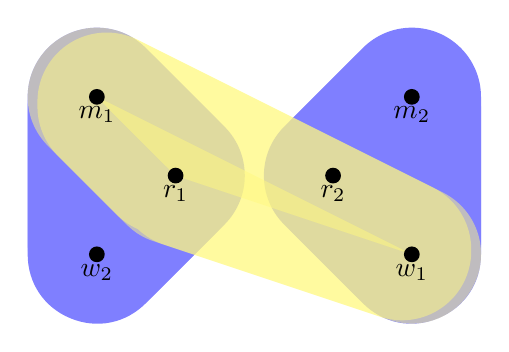
\begin{tikzpicture}
    \node (m1) at (-2,1) {};
    \node (m2) at (2,1) {};
    \node (w2) at (-2,-1) {};
    \node (w1) at (2,-1) {};
    \node (r1) at (-1, 0) {};
    \node (r2) at (1, 0) {};
    

    \tikzstyle{edge} = [fill,opacity=.4,fill opacity=.5,line cap=round, line join=round, line width=50pt]

    \begin{scope}[transparency group,opacity=.5]
    \draw[edge,opacity=0.5,color=blue] (m1) -- (r1) -- (w2) -- (m1);
    \filldraw[edge,opacity=1,color=blue] (m1.center) -- (r1.center) -- (w2.center) -- (m1.center);
    
    \draw[edge,opacity=0.5,color=blue] (m2) -- (r2) -- (w1) -- (m2);
    \filldraw[edge,opacity=1,color=blue] (m2.center) -- (r2.center) -- (w1.center) -- (m2.center);

    \draw[edge,opacity=0.5,color=yellow] (m1) -- (r1) -- (w1) -- (m1);
    \filldraw[edge,opacity=.5,color=yellow] (m1.center) -- (r1.center) -- (w1.center) -- (m1.center);
    \end{scope}

    
    \foreach \i in {1,2} {
        \fill (m\i) circle (0.1) node [below] {$m_{\i}$};
        \fill (w\i) circle (0.1) node [below] {$w_{\i}$};
        \fill (r\i) circle (0.1) node [below] {$r_{\i}$};
        
    }
\end{tikzpicture}

\subsection*{Other Properties}
We cannot guarantee that a stable matching always exists, or that the HyperCycle algorithm will generate one if it does exist. Moreover, it can be shown, as in the Pareto-Efficient Roommates Problem, that there does not exist a stable strategyproof mechanism for generating a Pareto-efficient matching. \cite{Morrill10}

\section*{Approximations and Heuristics}
A running theme in this paper is high difficulty. Both of our algorithms have exponential runtimes as a necessity. We ask what kind of approximations we can use to make these problems more tractable.

\subsection*{Rank-Order Approximations}
We ask how we can generate ``pretty good'' matchings with a feasible runtime. We discuss a few ways that we can simplify or shrink the problem in order to make it tractable. We mentioned earlier that splitting students into incompatible groups shrinks the binary FRP by a large factor. It isn't a huge mental leap for a college to first assign students to dorm buildings, and then choose rooms from there. Problems with genders aside, a floor of a building might house fifty students, which enters the realm of tractability. However, it would be more feasible to drop total Pareto-efficiency. 

\subsubsection*{Simplification to Swaps}
Let's discuss a version of efficiency where room trades cannot happen on cycles but must be direct swaps, much like the kidney exchange. Thanks to the weakness of Pareto-efficiency, we can actually generate a \textbf{pairwise-efficient} matching with a greedy algorithm. Iterate over all pairs of students, and swap them if all parties improve. Stop when no change occurs after iterating over all pairs. This algorithm has the advantage of being much simpler to understand and implement, and also allows preferences to be generated ad-hoc. That is, the HyperCycle Algorithm requires sorting all possible subsets (this process alone takes $\mathcal{O}(n^{k - 1})$ preferences per student), while the greedy algorithm presents pairwise comparisons only when necessary. 

A problem with algorithm is that it is quite easy to generate a bad matching. That is, what if you could allow two pairs of students to swap, but instead you take a path that only allows a single swap? We can improve our algorithm by first enumerating all possible swaps, then choosing the largest disjoint set of swaps. This would not greatly increase the runtime of the algorithm, and it is still guaranteed to terminate. This is still locally optimal only, just on a larger scale. Another possible improvement comes from the artificial intelligence technique of the decision tree. We could, for instance, select the single swap that gives an efficient matching among all possible matchings 5 steps in the future. However, this process is computationally very intense.

\section*{Conclusion}
Through discussion of this problem, we have scratched the surface of matching problem generalizations. Already we have seen that generalizing into hypergraphs causes an explosion of computational complexity. Due to this, we believe that heuristics and approximations are more worthy of study than exact algorithms. Heuristics are also far more useful in everyday scenarios. For example, it is ludicrous to ask students to sort even $\mathcal{O}(n)$ other roommates, let alone $n^2$ or more. There are also versions of these problems that could still be worth theoretic study, such as those involving multiple sets of students, or bisexual marriages, or other myriad other restrictions.

We believe that we have provided a starting point for investigation into both the exact and approximate versions of these problems. We believe our algorithms are correct, and that are approximations are believable. These approximations could also of course provide a starting point for humans to refine matchings. We have also provided evidence that, barring some huge leap in computational ability, humans will likely always be involved in problems of this sort. 

\begin{thebibliography}{9}
\bibitem{Morrill10}
    Thayer Morrill,
    \emph{The Roommates Problem Revisited}.
    Dept. of Economics, North Carolina State University,
    2010
\end{thebibliography}



\end{document}
